\documentclass[twocolumn,10pt]{article}
\usepackage[a4paper, top=0.5in, bottom=0.6in, left=0.5in, right=0.5in]{geometry}

\usepackage{graphicx}
\usepackage{algorithm}  
\usepackage{algorithmicx}  
\usepackage{algpseudocode}  
\usepackage{amsmath}
\usepackage{url}
\usepackage{xcolor}
\usepackage{listings}

\algnewcommand{\LeftComment}[1]{\Statex \(\triangleright\) #1}

\renewcommand{\algorithmicrequire}{\textbf{Input:}}  
\renewcommand{\algorithmicensure}{\textbf{Output:}}  
\graphicspath{{figure/}}

\begin{document}

\title{\bf Grouper: a Framework for Developing Mobile Applications using Secret Sharing and Untrusted Servers}

\author{
	Meng Li and Yasushi Shinjo \\
	University of Tsukuba
}

\maketitle

\begin{abstract}

This paper presents Grouper, a framework for developing mobile applications.
Grouper uses a secret sharing scheme to create several shares from a marshalled object and uploads these shares to multiple untrusted servers. 
These untrusted servers are a self-destruction system.
Uploaded shares will be deleted after a period of time.
Mobile devices exchange messages via untrusted servers based on the Grouper Message Protocol . 
We have implemented the Grouper framework for iOS, macOS, tvOS and watchOS in the Objective-C language.
We have implemented three applications using Grouper: an iOS application Account Book, a macOS application Notes and a benchmark application Test.
We evaluate the development efforts and the performance of Grouper. 
Experimental results show that the performance of Grouper is feasible for mobile applications that are used in a small group of people.

\end{abstract}

\textbf{Keywords: mobile application security, secret sharing, untrusted server}

\section{Introduction}

People use mobile applications everyday. 
Conventional mobile applications are built based on a client-server mode and require central servers for storing shared data and processing confidential information.
When users use such mobile applications, they must fully trust the central servers.
If the central servers are accessed by an attacker, a curious administrator or a government, private information will be revealed because data is often stored on the central servers in cleartext. 
In addition, users may lose their data when service providers shut down their servers.

To address such a problem, Vanish\cite{geambasu2009vanish}, SafeVanish\cite{zeng2010safevanish}, SeDas\cite{zeng2012sedas} and CouldSky\cite{zeng2015cloudsky} use a data self-destruction system as their cloud storage.
In these approaches, servers store data temporarily and delete data after a period of time.
Mylar\cite{popa2014building} and Sweets\cite{sweets} use data encryption to protect user data.
These existing approaches have following problems.
Firstly, they do not support data recovery when some nodes miss getting data from shared storage.
Application developers have to deal with such cases by themselves.
Secondly, these approaches do not support developing general mobile applications.

To address these problems, we are developing Grouper, a framework for developing mobile applications. 
Grouper provides object synchronization among mobile devices.
In Grouper, a sender node translates an updated object into shares using a secret sharing scheme and uploads these shares to untrusted servers. 
A receiver node downloads some of these shares and reconstructs the object.
The untrusted servers construct a self-destruction system, and delete these shares after a period of time.
We call it a Time To Live(TTL).
Unlike existing approaches, although Grouper uses the data self-destruction scheme, it support data recovery when some nodes miss getting shares from untrusted servers.
When a receiver node misses getting shares, the Grouper framework automatically asks the sender to upload missing shares again.
This scheme ensures reliable data sharing among devices of a group.
In addition, data can be recovered even untrusted servers shut down because all devices of a group keep a complete data set of this group.

Grouper consists of a client framework and a Web service.
We have implemented the Web service running on the multiple untrusted servers in Java. 
We have embedded a Sync framework in Grouper to synchronize objects among mobile nodes.
We have implemented three applications using Grouper: an iOS application Account Book, a macOS application Notes and a benchmark application Test.
These implementations shows that Grouper makes it easy to develop mobile applications with data synchronization.

The contributions of this paper are as follows.
Firstly, we provide support for data recovery when some nodes miss getting data from untrusted servers.
Grouper realizes reliable data synchronization among nodes using a reliable multicast technique.
Secondly, we make it easier to develop mobile applications.
A developer can add data synchronization functions to an applications with a few lines of code.

\section{Threat Model}

In this section, we introduce the assumptions and threat model underlying the Grouper framework.
We target mobile applications that are used in a small group of people.
A group consists of an owner and other members.
Each member has a mobile device.
A owner invites other members in a face-to-face way.

Firstly, a server is a passive adversary, and can read all data, but it does not actively attack.
The server hosts Web services and performs device authentication.
Servers generate access keys for group members. 
When a device wants to get/put data from/to untrusted servers, the device sends a request with an access key in the request header.
In this paper, we do not address other types of attack such as user tracking and metadata collection by servers. 
For example, the server can track users with IP addresses, and Grouper cannot hide social graphs against such tracking.

Secondly, data transportation between a device and an untrusted server is secure.
We can protect it using Transport Layer Security (TLS) or other encryption techniques.
Grouper focuses on privacy data storage in servers rather than data transportation.

Thirdly, in an application, all group members are not malicious and their devices connect to each other in a face-to-face distance.
We target applications that are used in a small group at the user invitation time.
For example, the group members are working in an office.
They know one another and they are not malicious.
When a group owner invites new members, the owner authenticates group members by a face-to-face way.

At last, a server is isolated from one another and managed by independent providers.
We assume that providers of untrusted servers do not expose users' data to other providers.
For example, a group owner can pick up servers of Amazon, Google, and Microsoft, which are supposed not to expose users' data to other cloud providers.

\section{Design}

This section describes the design of the Grouper framework.

\subsection{Overview}

Our goal is to support developing mobile applications that are not relying on trusted central servers.


To support developing such mobile applications, we provide the Grouper framework.
This framework provides the following functions:

\begin{itemize}
	\setlength{\itemsep}{1pt}
	\setlength{\parskip}{0pt}
	\setlength{\parsep}{0pt}
	\item \textbf{Data Synchronization.} 
	If an user updates or deletes an object in his device, the mirrors of this object in other devices are updated or deletes.
	\item \textbf{Group management.} 
	A group owner can create a group and invite other members to his group.
\end{itemize}

For example, \emph{Account Book} is an iOS application developed using Grouper. 
In this application, a leader of a small company creates a group and invites employees to the group. 
Then, the employees can record the income and expenditure of this company and share these records to others.
Anyone can edit and delete existing records.

Grouper uses untrusted servers to exchange messages among mobile devices.
Untrusted servers construct a self-destruction system, and delete messages after a TTL.

Grouper protect messages from the providers of untrusted servers using a secret sharing scheme.
Grouper uses Shamir's secret sharing scheme to protect user data rather than data encryption methods.
In  Shamir's secret sharing scheme, a member securely shares a secret with other members by generating $n$ shares using a cryptographic function\cite{smith2013layered}. 
At least $k$ or more shares can reconstruct the secret, but $k-1$ or fewer shares can obtain nothing about the secret\cite{pang2005new}. 
We describe this scheme as a function ${f(k, n)}$, where $n$ is the number of all shares, and $k$ is the threshold to combine shares. 

Grouper has the following advantages over conventional systems using untrusted servers.
Firstly, it is easy for a developer to recover from message losses in untrusted servers (Section 3.4).
Grouper performs retransmission when some mobile devices miss getting messages from untrusted servers.
Developers of mobile applications do not have to specify lifetimes of messages.
Secondly, it is easy for a group owner to invite other members using a safe communication channel in a face-to-face distance (Section 3.7).

\subsection{Architecture}

\begin{table*}[t]
	
	\centering
	\caption{Client API of Grouper.}
	\label{my-label}
	\begin{tabular}{ll}
		\hline
		\textbf{Method} & \textbf{Description} \\ \hline
		grouper.\textbf{setup}(appId, dataStack) & 
		\begin{tabular}{@{}l@{}}
			This method setups Grouper with appId and dataStack. AppId is a unique ID of\\ an application. Datastack is used by the synchronization plugin. \\
		\end{tabular}  \\ \hline
		grouper.sender.\textbf{update}(object) & 
		\begin{tabular}{@{}l@{}}
			An application invokes this method after creating a new object or modifying an\\ existing object. Grouper performs updating asynchronously and sends an update\\ message to other devices.
		\end{tabular} \\ \hline
		grouper.sender.\textbf{delete}(object) & 
		\begin{tabular}{@{}l@{}}
			An application invokes this method when the application wants to delete an existing\\ object. Grouper will delete the object and remove it in the persistent store of a\\ device automatically after sending a message to other devices.
		\end{tabular} \\ \hline
		grouper.receiver.\textbf{receive}(callback) & 
		\begin{tabular}{@{}l@{}}
			An applications invokes this method to register the callback function that is called\\ after Grouper processes received messages and update objects according to the\\ messages. The application can use this callback function to update the user screen. 
		\end{tabular} \\ \hline
		grouper.sender.\textbf{confirm}() & 
		\begin{tabular}{@{}l@{}}
			An application needs to invoke this method periodically or occasionally to send\\ confirm messages to other devices.
		\end{tabular} \\ \hline
	\end{tabular}
\end{table*}

\begin{table*}[t]
	\centering
	\caption{The API of the synchronization plugin.}
	\label{my-label}
	\begin{tabular}{ll}
		\hline
		\textbf{Method} & \textbf{Description} \\ \hline
		marshall(o) & Marshalls the object o and returns the marshalled byte array. \\
		sync(b) & Unmarshalls the byte array b to the object and puts the object into the persistent store. \\ \hline
	\end{tabular}
\end{table*}

\begin{figure}[t]
	\centering
	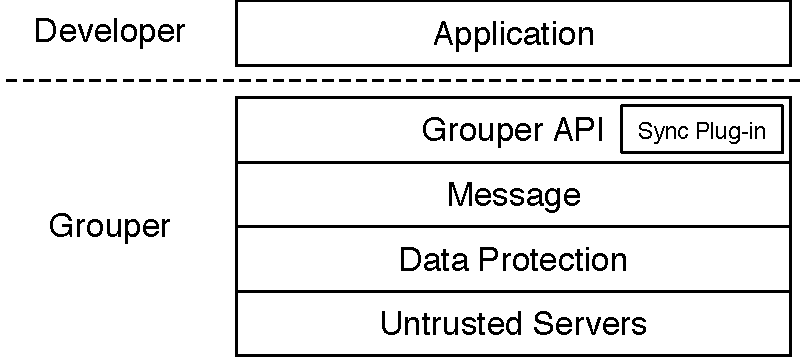
\includegraphics[scale=0.45]{architecture}
	\caption{Architecture of Grouper.}
\end{figure}

Figure 1 describes the architecture of the Grouper framework. 
An application using Grouper consists of the six following layers:

\begin{itemize}
	\setlength{\itemsep}{1pt}
	\setlength{\parskip}{0pt}
	\setlength{\parsep}{0pt}
	\item \textbf{Grouper API}
	A developer develops an application without data synchronization at first. 
	He adds the synchronization function to his application by using this API.
	\item \textbf{Synchronization Plugin.} 
	Grouper uses a third-party framework for data synchronization.
	This layer marshalls an updated object in a persistent store and sends it using the lower reliable message layer.
	When this layer receives a message, this layer unmarshalls the message, reconstructs an object, and puts the object into the persistent store.
	\item \textbf{Message.}
	This layer provides a message service with multicasting capability among devices.
	The destination of a massage is not only the node identifier (ID) of a single device but also "*", which means delivering to all the other nodes.
	This layer does not ensure the message delivery to other devices.
	\item \textbf{Data Protection.}
	Grouper protects user data by a secret sharing scheme in this layer.
	This layer divides a message into several shares, and uploads these shares to untrusted servers.
	When this layer downloads shares from untrusted servers, it recovers the original message using the secret sharing scheme.
	\item \textbf{Untrusted servers.}
	When a mobile device uploads a share to an untrusted server, this server receives it and stores it into a database.
	When a mobile device downloads a share from an untrusted server, this server retrieves it from the database and send it into the device.
	An untrusted server performs device authentication using device keys.
\end{itemize}

The following subsections describe details of these layers from the top layer to the bottom layer.

\subsection{Grouper API}

The Grouper framework provides object synchronization among mobile devices through put a simple client API.
A developer can add object synchronization functions to a standalone application with a few lines of code.
Table 1 shows the client API of Grouper.
An application initializes the framework by invoking the method $grouper.setup()$.
When the application needs to update an object in all devices, the application invokes the method $grouper.sender.update()$.
When the application needs to delete an object in all devices, the application invokes the method $grouper.sender.delete()$.
The the application uses the method $grouper.receiver.receive()$ to register a callback function.
This callback function is called when another node updates an object and its local mirror has been updated.
The application can use this callback function to change the values that are shown in a user interface screen.
The method $grouper.confirm()$ is used for realizing reliable messaging.
We will describe reliable messaging in Section 3.4.

The Grouper API layer relies on two modules: the synchronization plugin and the reliable messaging layer.
When an object is updated in a local device, the synchronization plugin marshalls an updated object and returns a message.
Next, the Grouper API layer sends this messages using the reliable messaging layer.
When an object is updated in an other device, the Grouper API layer receives a message using the reliable messaging layer.
Next, the Grouper API layer updates the object by passing the received message to the synchronization plugin.

We have not implemented the synchronization plugin by ourselves, but we make this layer as a pluggable module.
This is because there are many such synchronization modules that provide various features, and application requirements also vary.
Each application developer should choose a suitable module based on a consistency model and other requirements.
As described in Table 2, the synchronization plugin should provide the $marshall(o)$ and $sync(b)$ functions.
Grouper invokes them to get marshalled data from the persistent store and save unmarshalled data into the persistent store.

Because we implement our client framework in Objective-C at first, we use the Sync framework\cite{sync} to implement a data synchronization plugin currently.
The Sync framework marshalls objects into JavaScript Object Notation (JSON) strings and provides a consistency model where the newest edition wins.

\subsection{Reliable Message Delivery}

Grouper realizes reliable message delivery over the self-destruction system in the Grouper API layer.

To design this, we use a reliable multicasting technique in distribute systems\cite{tanenbaum2007distributed}.
In this reliable multicasting technique, each message has a sequence number for each sender.
Each member keeps the newest sequence numbers for senders and detects missing messages.
If a member notices missing a message from a sender, the member asks the sender to resend the message.
For example, consider that a sender sends Message No.3 to all other members using a multicast address.
When a member receives this Message No.3, the member compares the sequence number 3 with the newest sequence number of the sender.
If the the newest sequence number of the sender is 1, this means the member missed Message No.2.
The member asks the sender to resend Message No.2.
The sender will send Message No.2 to the asked member using a unicast address.

This basic reliable multicasting technique works well for continuous medias, such as video streaming in Internet communication.
However, this does not work if receivers become often offline for a long time and servers delete messages soon.

To address this problem, we design our own reliable messaging by extending the basic reliable multicasting technique.
We use special types of messages that include active sequence numbers.
Using these messages, a receiver can easily know missing messages.

This idea is inspired from the checkgroups message of Usenet\cite{usenet}.
In Usenet, the list of active newsgroups is maintained with two basic messages: newgroup and rmgroup.
When a node receives a newgroup message, the node adds the newsgroup to the list.
When a node receives a rmgroup message, the node removes the newsgroup from the list.
These basic messages can be lost and the list can be obsolete.
Ckeckgroups message messages supplement these basic messages.
A checkgroups message includes the list of all newsgroups in a newsgroup hierarchy.
A checkgroups message is distributed periodically or after some time after basic messages are distributed.

\begin{figure}[t]
	\centering
	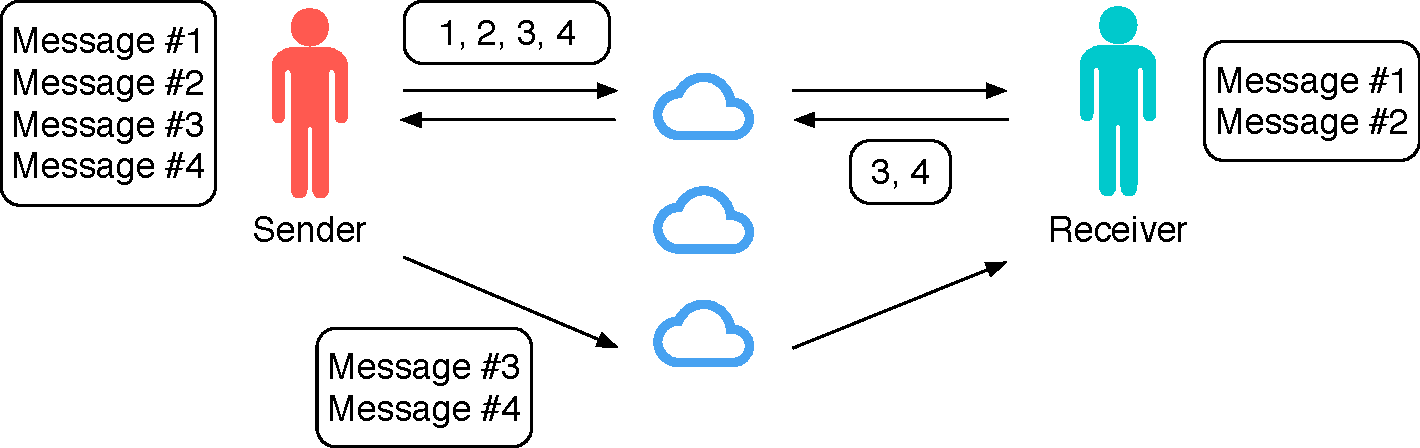
\includegraphics[scale=0.38]{reliable_sync}
	\caption{Implementing reliable messaging with continuous sequence numbers.}
\end{figure}

Figure 2 shows that the sender is sending five messages from No.1 to No.5 to the receiver.
The sender uploads two messages, No.1 and No.2 using a multicast address.
The receiver downloads these two messages and becomes offline.
The servers delete these two messages.
The sender uploads next three messages from No.3 and No.5  using a multicast address.
The receiver becomes online, but the receiver does not notice that the receiver has missing messages soon.
At this time, the sender sends a special message that includes the newest active sequence number No.5.
The receiver receives these sequence numbers and compares them with the newest sequence number in the persistent store.
In Figure 3, the receiver notices that Messages No.3, No.4 and No.5 are missing.
The receiver asks the sender to resend Messages No.3, No.4 and No.5.
The sender will send Messages No.3 and No.4 to the receiver again using a unicast address.

\subsection{Unreliable Messaging}

This subsection describes the design of unreliable messaging in the layers of Messaging, Data Protection, and Untrusted Servers.

In these layers, we use a secret sharing scheme and multiple untrusted servers as shown in Figure 3.
In this figure, the messaging layer in the sender is sending a message to that in the receiver.

At first, this layer calls the data protection layer and creates three shares by a secret sharing scheme.
Next, this layer uploads those shares to three untrusted servers.
Each untrusted server receives one of these shares and stores it into a database.

\begin{figure}[t]
	\centering
	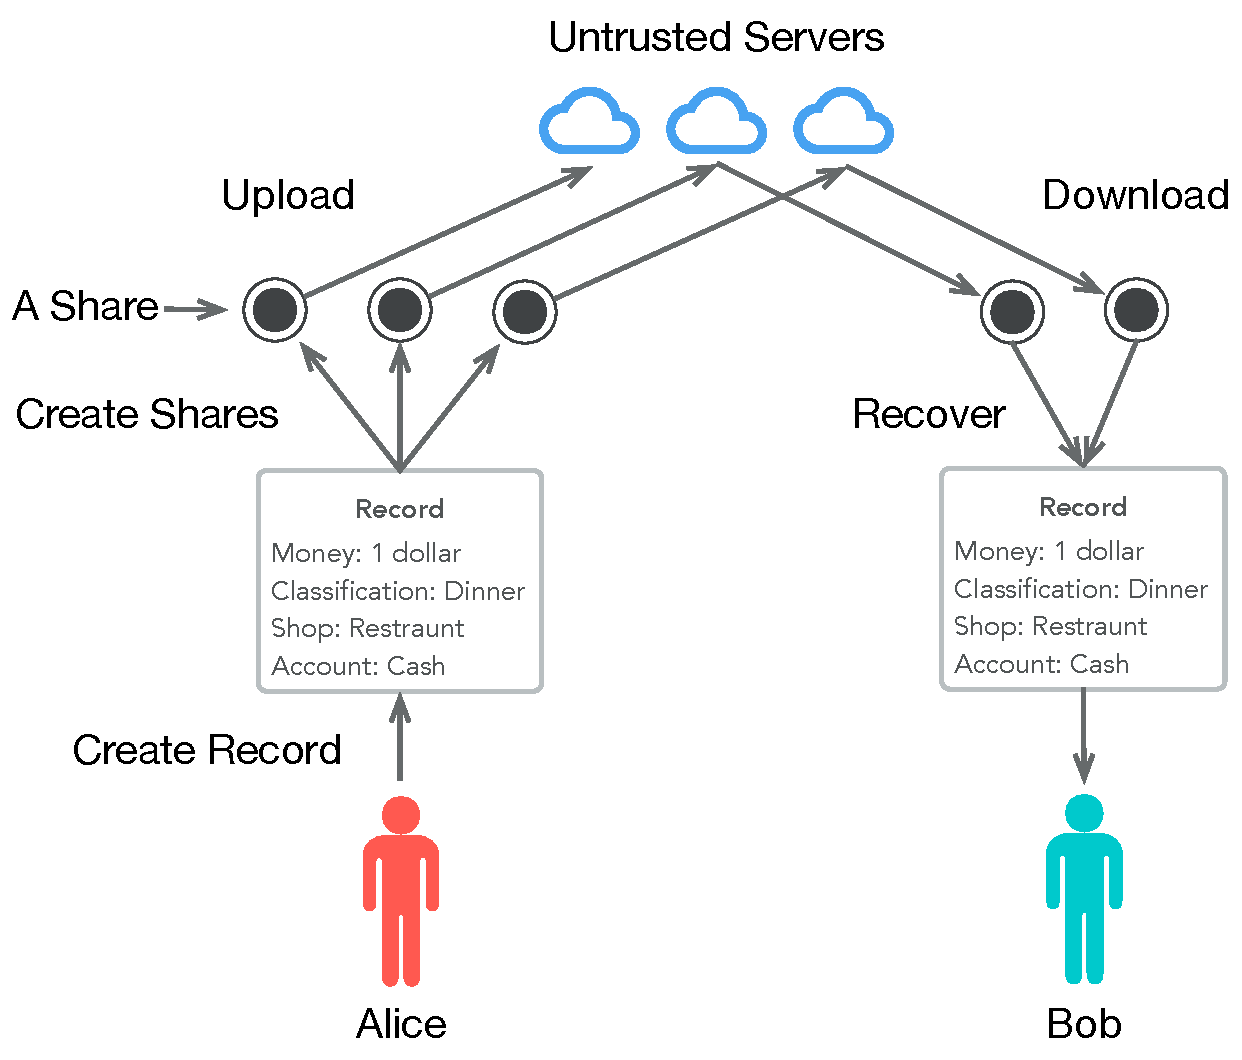
\includegraphics[scale=0.42]{sync_flow}
	\caption{Implementing unreliable messaging with a secret sharing scheme and multiple untrusted servers.}
\end{figure}

In Figure 3, the receiver is online, and its messaging layer downloads two shares from two servers.
Next, this layer calls the the data protection layer and recovers the message from these two shares using the secret sharing scheme.
Finally, the messaging layer in the receiver puts the message to the upper layer, the reliable message layer.

The data protection layer uses the Shamir's secret sharing scheme $f(k, n)$ introduced in Section 3.1 to protect a message from untrusted servers.
In this scheme, a message is divided into $n$ shares using a cryptographic function.
A receiver gets more than $k$ shares to combine them to original message.

In Grouper, we use our new scheme $ f(k, n, s)$ by extending the scheme $f(k, n)$.
In our scheme, the parameter $k$ and $n$ are same as these in the scheme $f(k, n)$. 
The parameter $s$ represents the minimum number of untrusted servers when a sender uploads shares, where $k \leq s \leq n$.
Although a receiver is able to recover the original message from at least $k$ shares, we should consider server crashing. 
When a sender uploads $n$ shares to $n$ untrusted servers successfully, Grouper will try to upload these $n$ shares to all $n$ untrusted servers at first. 
If the shares are uploaded to $s$ or more untrusted servers, we consider that this share uploading is successful.
Otherwise, Grouper keeps trying to upload these shares.

\subsection{Grouper Message Protocol}

\begin{table}[t]
	\centering
	\caption{Attributes of Grouper message.}
	\label{my-label}
	\begin{tabular}{lll}
		\hline
		\textbf{Attribute} & \textbf{Explanation} \\ \hline
		type & Type of this message. \\
		content & A marshalled object or sequence numbers. \\
		sequence & Sequence number of this message. \\
		class & Class name of an object. \\
		objectId & Physical ID of an object. \\
		receiverId & Node identifier of the receiver. \\
		senderId & Node identifier of the sender. \\
		email & Email address of the sender. \\
		name & Name of the sender. \\
		sendtime & Unix timestamp of sendtime. \\
		\hline
	\end{tabular}
\end{table}

The Grouper API layer sends and receives messages using our own protocol, Grouper Message Protocol.
In this protocol, a message is a JSON string that contains a marshalled object and attributes.
Table 3 shows the attributes in a Grouper message.
There are three important attributes:

\begin{itemize}
	\setlength{\itemsep}{1pt}
	\setlength{\parskip}{0pt}
	\setlength{\parsep}{0pt}
	\item \textbf{Type.}
	This attribute means types of messages.
	There are four types of messages: update messages, delete messages, confirm messages and resend messages.
	An update message contains the marshalled objects of an application.
	A delete message contains the physical identifier of a deleted object.
	We call update messages and delete messages \emph{normal messages}. 
	Both confirm message and resend message contain control information about reliable multicast. 
	We call these messages \emph{control messages}.
	\item \textbf{Content.} 
	If this message is an update message, the content value contains the JSON string of a marshalled object.
	If this message is a delete message, the content value contains the objectId of an object.
	If this message is a confirm message, the content value contains maximum sequence number of messages created in the device of the sender.
	If this message is a resend message, the content value contains the range of missing messages' sequence numbers.
	\item \textbf{Sequence.}
	This attribute means the sequence number of the message.
	When a sender sends a new normal message, the sender increments the sequence number and includes it to the new message.
	The sequence number of any control message is 0, because it need not to be resent.
	Using both the sequence number and the ID of the sender identify a unique message.
\end{itemize}

The attribute receiverId contains the addresses of destination devices.
An address is either a list of device IDs or ``*'' that means multicasting to all devices.

\begin{algorithm}[t]
	\caption{Handle message algorithm}\label{alg:euclid}
	\begin{algorithmic}[1]		
		\Procedure{onMessageReceived}{$msg$}
		\LeftComment Check duplicate message.
		\State  $historyMsgs \gets getMsgsBySender(msg.sender)$
		\If{$msg \in historyMsgs$}
		\State \textbf{return}
		\EndIf
		\State $lastMsg \gets historyMsgs.last()$
		\State $historyMsgs.add(msg)$
		 
		\LeftComment Begin basic reliable multicast.
		\If{$ msg.seq != 0 \ \&\& \ lastMsg.seq + 1 != msg.seq$}
		\State $resendMsg \gets createResendMsg(lastMsg.seq + 1, msg.seq)$
		\Comment Create a resend message by the minimum and maximum sequence number.
		\State $sendMsg(resendMsg)$
		\EndIf
		
		\LeftComment Handle the message by its type.
		\If{$msg.type = "update"$}
		\State $sync.updateRemote(msg)$
		\ElsIf{$msg.type = "delete"$}
		\State $sync.deleteRemote(msg)$
		\ElsIf{$msg.type = "confirm"$}
		\State $maxSeq = getMaxSeqFrom(msg.content)$
		\State $resendMsg \gets createResendMsg(lastMsg.seq + 1, maxSeg)$
		\State $sendMsg(resendMsg)$
		\ElsIf{$msg.type = "resend"$}
		\State $seqs \gets getSeqs(msg.content)$
		\For{$\forall seq \in seqs$}
		\State $missingMsg \gets getMsg(seq)$
		\State $sendMsg(missingMsg)$
		\EndFor
		\EndIf
		\EndProcedure
	\end{algorithmic}
\end{algorithm}

Applications send update, delete and confirm messages through the Grouper API and send resend messages after receiving messages automatically.
When the applications invoke the method $grouper.sender.update()$ of the Grouper API, the Grouper API layer sends an update message that contains the marshalled object to all devices.
When the applications invoke the method $grouper.sender.delete()$ of the Grouper API, the Grouper API layer sends a delete message that contains the ID of the deleted object to all devices. 
When the applications invoke the method $grouper.confirm()$, the Grouper API layer sends a confirm message to all devices. 
This confirm message includes the sequence numbers of objects that are recently created in this device.
Generally, the method $grouper.confirm()$ is invoked at the following occasions:

\begin{itemize}
	\setlength{\itemsep}{1pt}
	\setlength{\parskip}{0pt}
	\setlength{\parsep}{0pt}
	\item \textbf{Periodically.}
	For example, an application sends a confirm message now, and it will try to send a confirm message after the TTL because the shares of normal messages are deleted in untrusted servers after the TTL.
	\item \textbf{After the device becomes online.} 
	Sometimes, a device is offline and cannot send a confirm message after the TTL.
	Grouper sends a confirm message when this device becomes online.
\end{itemize}

Algorithm 1 describes the handle process when the Grouper API layer receives a message.
For an update message or a delete message, Grouper invokes the method $sync.updateRemote()$ or $sync.deleteRemote()$ of the synchronization plugin to put the modification of this object into the persistent store.
For a confirm message, the Grouper API layer creates the sequence numbers from the message content and removes those sequence numbers which exist in the device.
Next, the Grouper API layer creates a resend message that contains the missing sequence numbers and sends it to the sender of this confirm message.
For a resend messages, the Grouper API layer gets the sequence numbers, finds the corresponding normal messages and send them to the sender of this resend message.

\subsection{Group Management}

To manage a group, Grouper provides the following two functions:

\begin{itemize}
	\setlength{\itemsep}{1pt}
	\setlength{\parskip}{0pt}
	\setlength{\parsep}{0pt}
	\item \textbf{Group Creation.}
	A user creates a group, and he becomes the owner of this group.  
	Before creating a group, the owner prepares his own user information including his email and name, multiple untrusted servers, a group ID and a group name. 
	Next, he initializes this group on all untrusted servers by submitting his node identifier, the parameters of scheme $f(k, n, s)$ and the TTL. 
	The node identifier, which represents his device, is generated by Grouper randomly when the application is launched at the first time. 
	In each untrusted server, the Web service initializes this new group and returns a master key including the highest privilege to the owner. 
	The owner can add other members to an untrusted server by the master key.
	\item \textbf{Member Invitation.} 
	After creating a group, the owner can invite a new member to his group. 
	To join the group, a new member prepares his user information at first. 
	The owner invites the new member by a face-to-face way rather than using central servers. 
	At this time, Grouper establishes connection between their devices using a local safe communication channel like \emph{Multipeer Connectivity}\cite{mc}. 
	Firstly, the new member sends user information and a node identifier to the owner. 
	The owner saves the user information and the node identifier to his device. 
	Secondly, the owner registers the new member to multiple untrusted servers by submitting the node identifier of the new member. 
	Thirdly, untrusted servers return access keys for the new member to the owner. 
	Lastly, the owner sends the access keys, server addresses and the list of existing members to the new member. 
	After receiving them, the new member can access these untrusted servers with the keys.
\end{itemize}

\begin{table*}[t]
	\small
	\centering
	\caption{Applications' lines of code.}
	\label{my-label}
	\begin{tabular}{cccccc}
		\hline
		\textbf{Application} & \textbf{Platform} & \textbf{Lanaguage} & \textbf{Number of Entities} & \textbf{Standalone Application LoC} & \textbf{Increased LoC} \\ \hline
		Account Book & iOS & Objective-C & \multicolumn{1}{r}{5} & \multicolumn{1}{r}{8076} & \multicolumn{1}{r}{190} \\ 
		Notes & macOS & Swift & \multicolumn{1}{r}{5} & \multicolumn{1}{r}{???} & \multicolumn{1}{r}{???} \\
		Test & iOS & Swift & \multicolumn{1}{r}{1} & \multicolumn{1}{r}{621} & \multicolumn{1}{r}{18} \\  \hline 
	\end{tabular}
\end{table*}

\section{Implementation}

Grouper consists of a Web service running on multiple untrusted servers and a client framework for developing mobile applications.
We describe the implementation of the Web service (Section 4.1), the implementation of the client framework (Section 4.2) and demo applications (Section 4.3) in this section.

\subsection{Web Service}

We have chosen implementing own Web service rather than using commercial general cloud services like Amazon Simple Storage Service (S3), Google Cloud Storage, and Microsoft Azure Storage for the following reasons:

\begin{itemize}
	\setlength{\itemsep}{1pt}
	\setlength{\parskip}{0pt}
	\setlength{\parsep}{0pt}
	\item The Web service must support on the Grouper Message protocol.
	\item The Web service must delete shares after a prescriptive time.
\end{itemize}

Our Web service provides a RESTful API to clients.
It runs on the Tomcat server that is an open source implementation of the Java Servlet, JavaServer Pages, Java Expression Language and Java WebSocket technologies\cite{tomcat}. 
We use the Spring MVC, a  Web model-view-controller framework, to create our RESTful API\cite{spring}, and Hibernate, an open source Java Object-Relational Mapping (ORM) framework, to save and operate objects in the Web service\cite{hibernate}. 

Our Web service includes three kinds of entities: \emph{Group}, \emph{User} and \emph{Share} entities. 
A \emph{Group} entity saves a group ID, a group name and its owner. 
A \emph{User} entity saves the node identifier of a user, the access key for this user, and the group entity of this user. 
A \emph{Share} entity saves a share generated with the secret sharing scheme, the time when a client uploads the share. 

\subsection{Client Framework}

Grouper's client framework is written in Objective-C, and it supports developing applications on iOS, macOS, watchOS and tvOS.
It makes use of the following frameworks.   

\begin{itemize}
	\setlength{\itemsep}{1pt}
	\setlength{\parskip}{0pt}
	\setlength{\parsep}{0pt}
	\item 
	\emph{Multipeer Connectivity}\cite{mc},  an official Peer-to-Peer communication framework provided by Apple. 
	Grouper uses it to transfer data between two devices by a face-to-face way.
	\item 
	\emph{Core Data}\cite{coredata}, an official ORM framework provided by Apple.
	\emph{Core Data} provides generalized and automated solutions to common tasks associated with object life cycles and object graph management, including persistence. 
	Grouper uses it to manage model layer objects. 
	\item 
	\emph{Sync}, a synchronization framework for \emph{Core Data} using JSON. 
	This framework marshalls objects into JSON strings and vice versa. 
	Grouper uses it in the synchronization plugin.
	\item 
	\emph{c-SSS}\cite{c-sss}, an implementation of the secret sharing scheme.
	\item 
	\emph{AFNetworking}\cite{afnetworking}, a networking library in Objective-C. 
	Grouper uses it to invoke the RESTful API provided by our Web services running on multiple untrusted servers. 
\end{itemize}

\subsection{Application}

\begin{figure}[t]
	\centering
	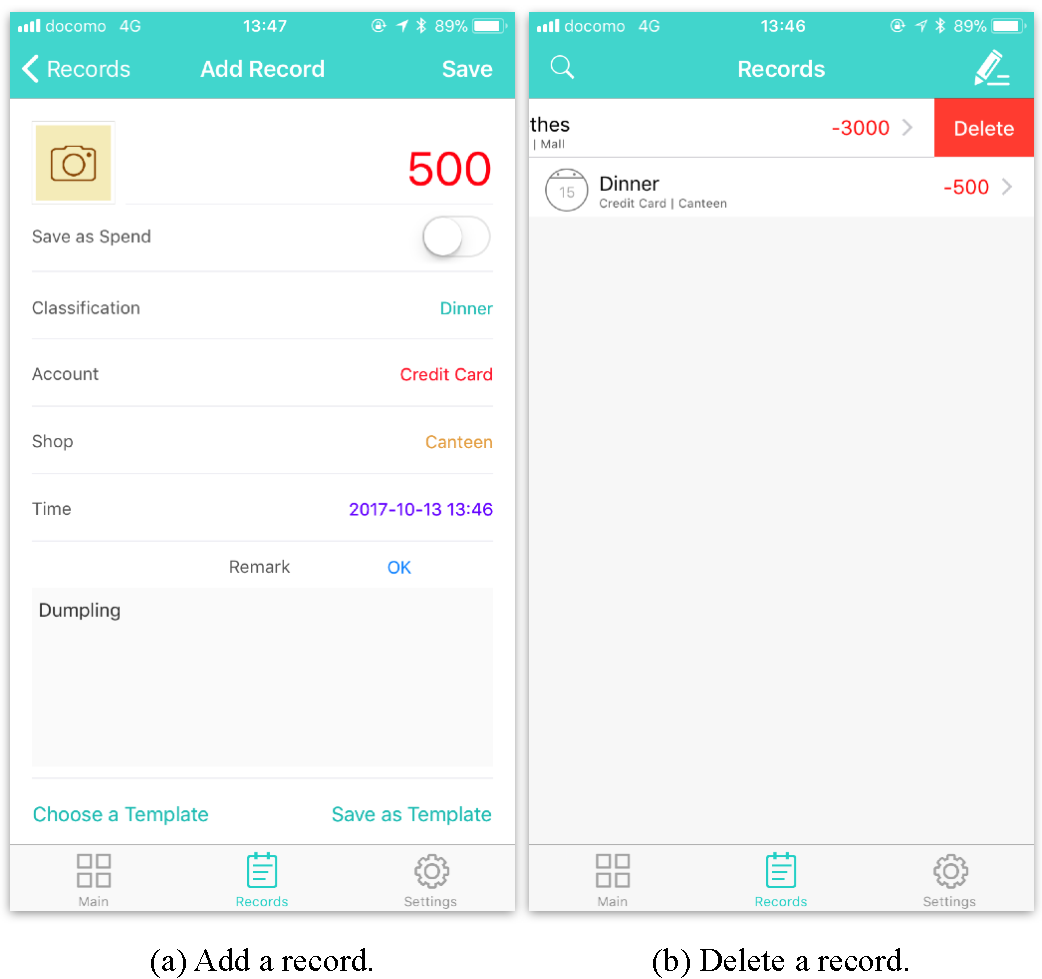
\includegraphics[scale=0.5]{account_book}
	\caption{Screenshots of demo application Account Book.}
\end{figure}

Using the Grouper framework, we have developed the following applications. 

\begin{itemize}
	\setlength{\itemsep}{1pt}
	\setlength{\parskip}{0pt}
	\setlength{\parsep}{0pt}
	\item \emph{Account Book}, an iOS application in Objective-C, records the income and expenditure of a group.
	\item \emph{Notes}, a macOS application in Swift, takes shared notes for a small group.
	\item \emph{Test}, a benchmark iOS application in Swift, tests the performance of Grouper.
\end{itemize}

Figure 4(a) shows the screenshot of adding a record in Account Book. 
A user uses Account Book to add income and expenditure records that include classification, account, shop, time and remark of a group. 
When the user click the save button, Account Book invokes the $grouper.sender.update(object)$ method of Grouper to share this record to other group members.
Figure 4(b) shows the screenshoot of deleting a record in Account Book. 
A user can swipe a cell from right to left to delete a record in the record list. 
When the user click the delete button, Account Book invokes the $grouper.sender.delete(object)$ method of Grouper to delete this record on the devices of other group members.

\begin{figure*}[t]
	\centering
	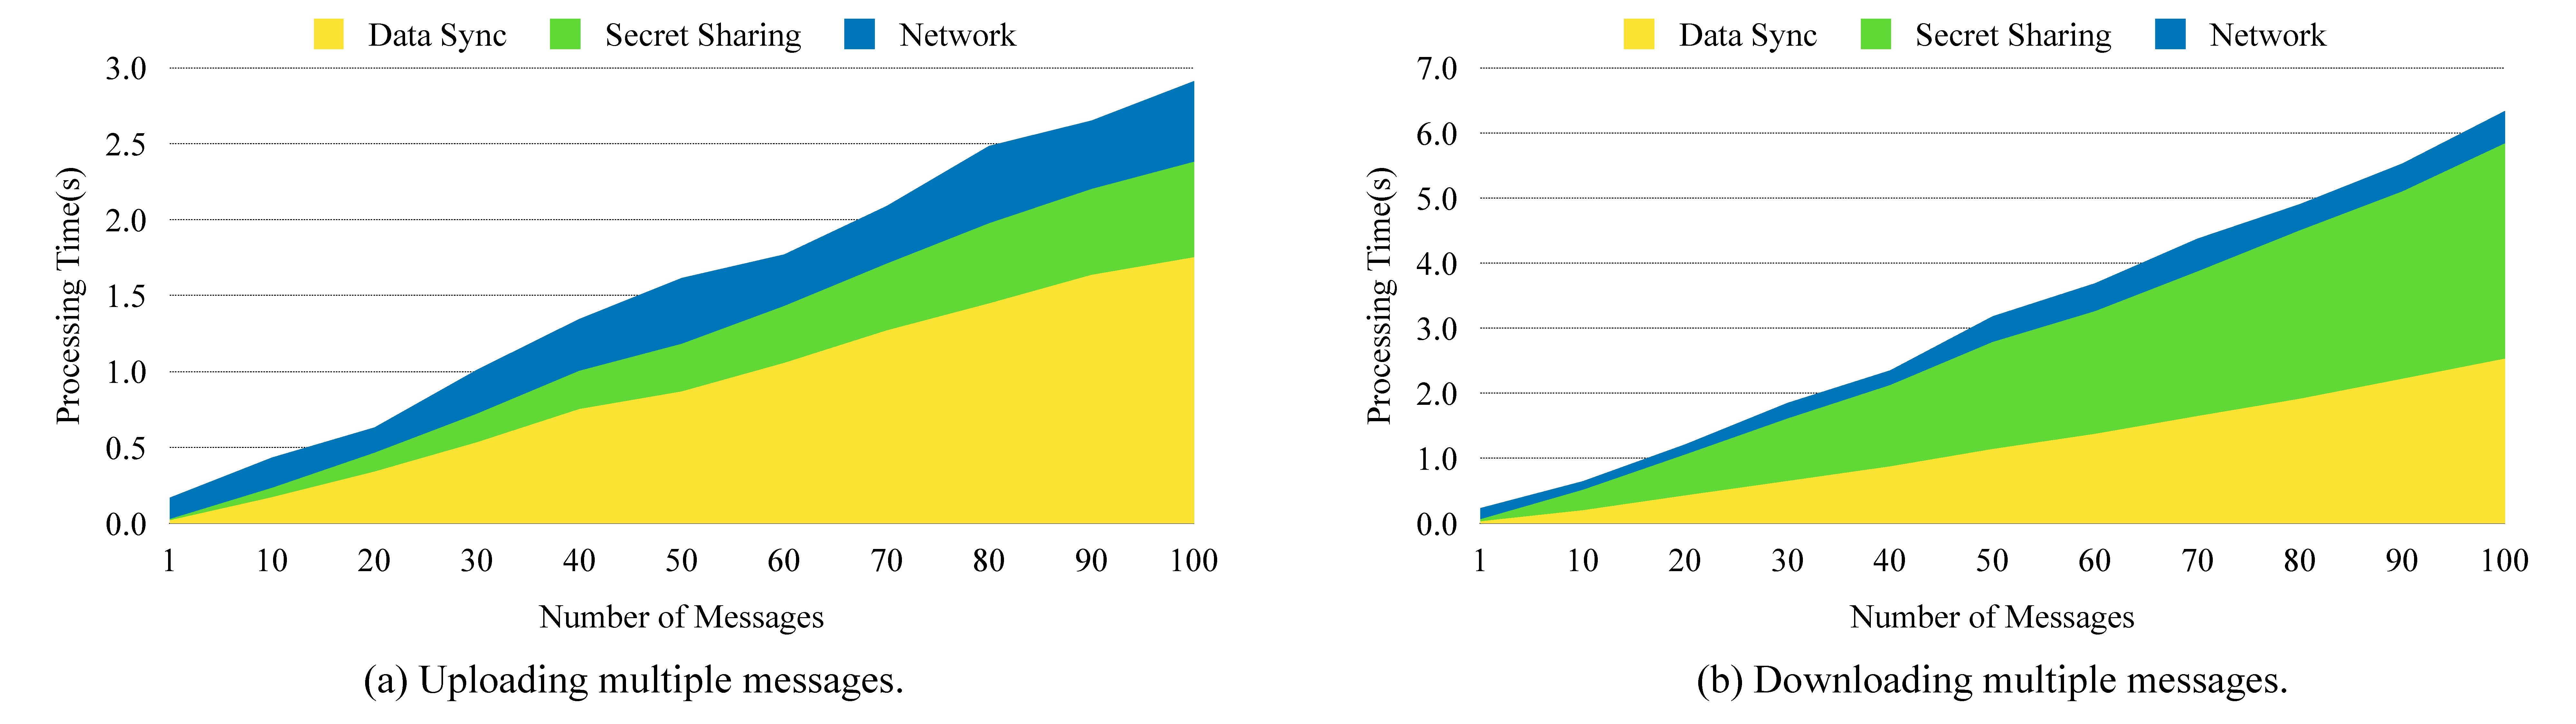
\includegraphics[scale=0.13]{multiple_messages}
	\caption{Processing time of sending and receiving multiple messages.}
\end{figure*}

\begin{figure*}[t]
	\centering
	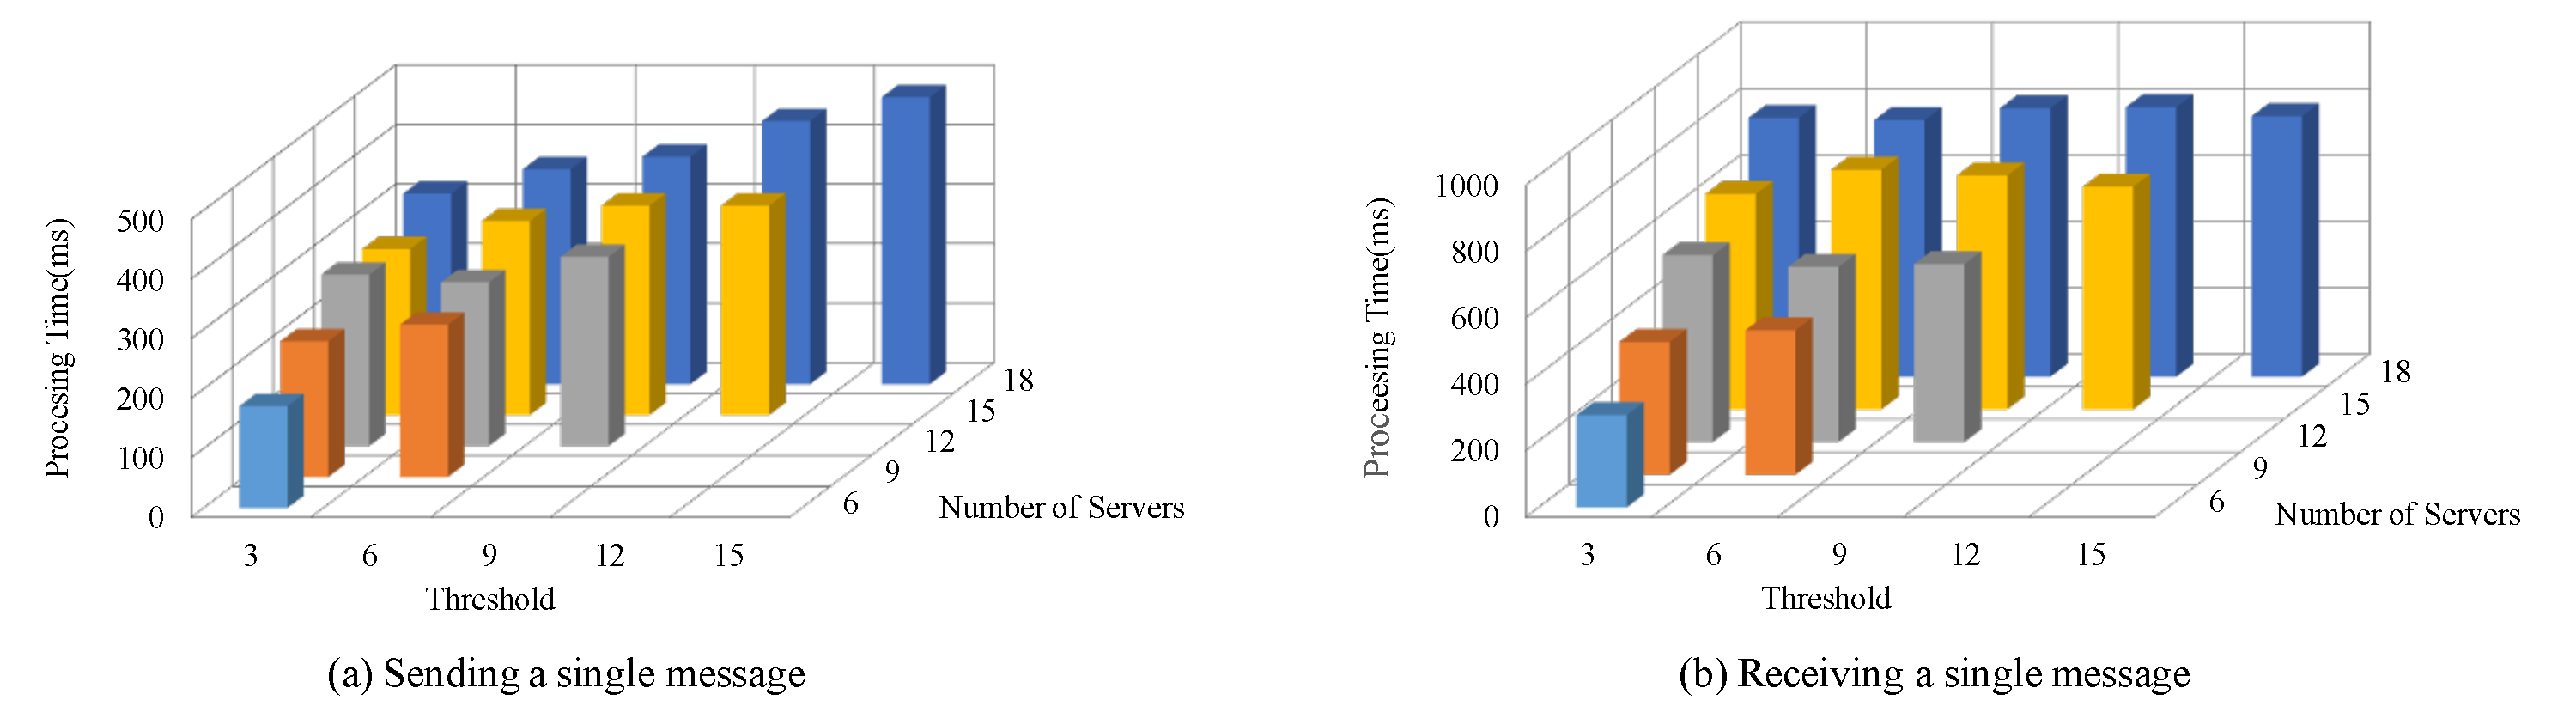
\includegraphics[scale=0.35]{3d}
	\caption{Processing time of sending and receiving a single message with different scheme.}
\end{figure*}

\begin{figure*}[t]
	\centering
	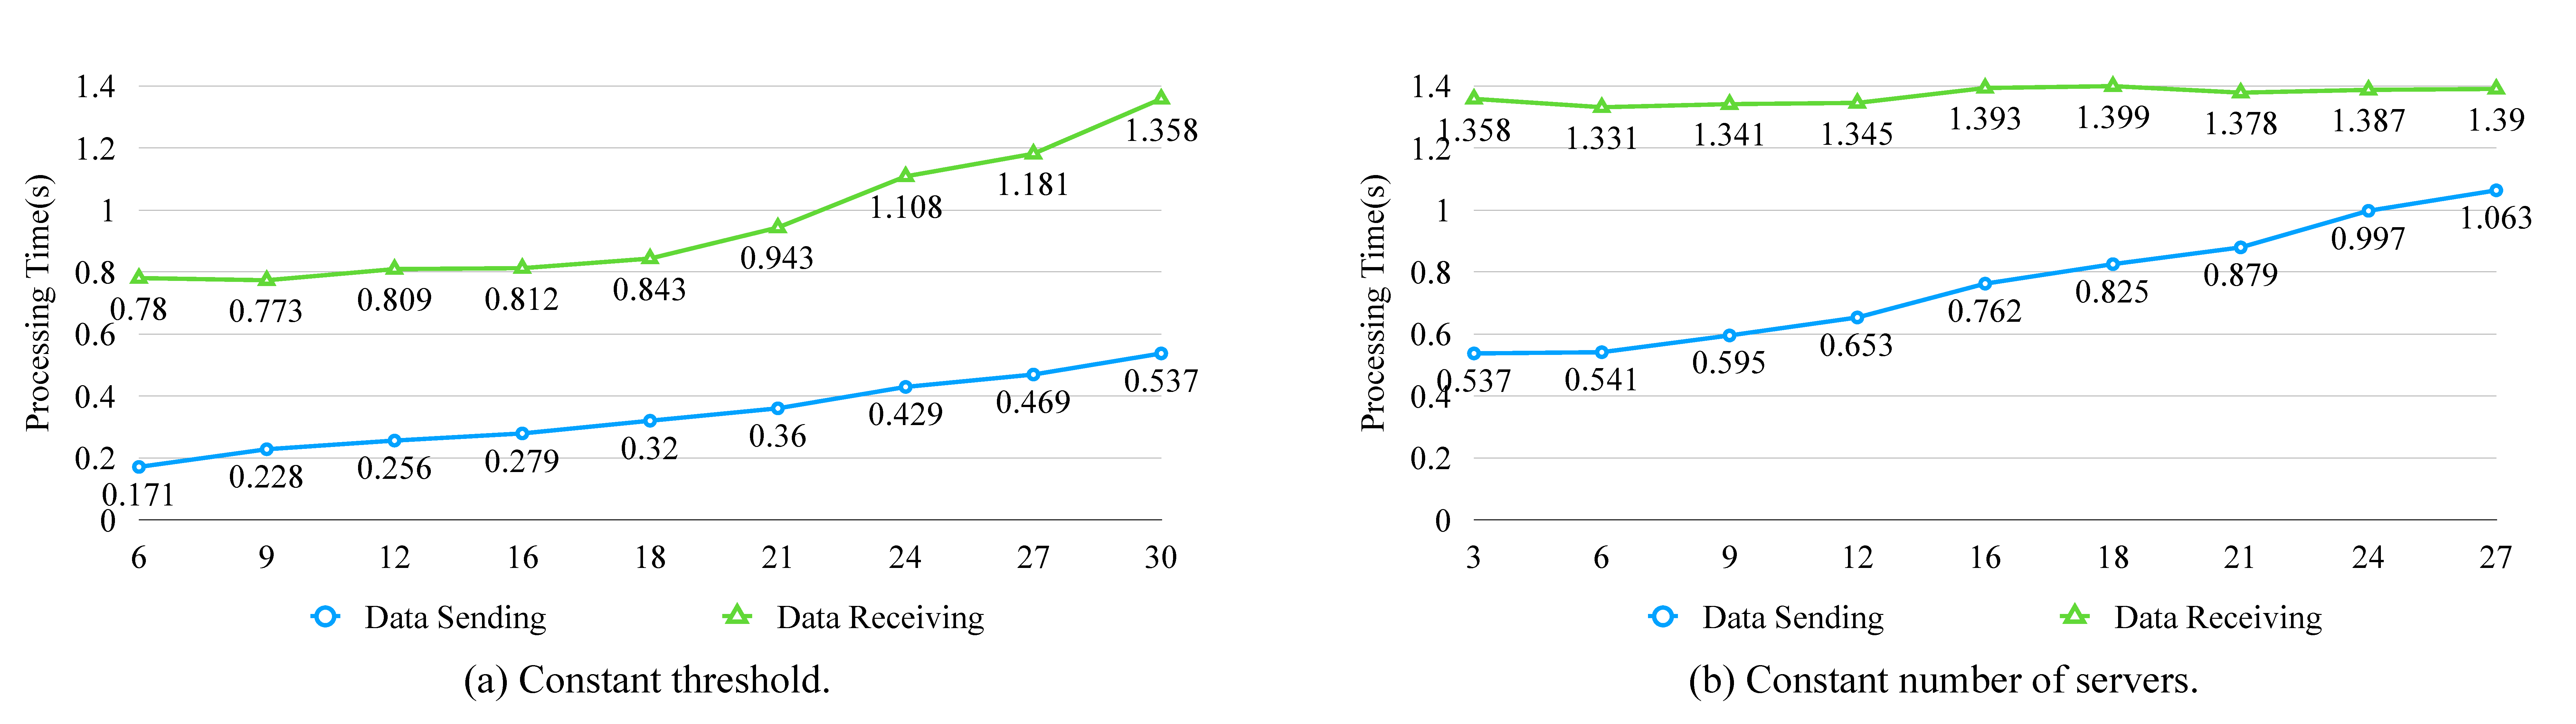
\includegraphics[scale=0.13]{constant_k_n}
	\caption{Processing time of sending and receiving a single message with a constant ${k}$ or ${n}$.}
\end{figure*}

\section{Evaluation}

This section shows the development efforts to use Grouper and the performance of Grouper.

\subsection{Development Efforts}

We see development efforts through two factors: the usability of the client API and the code size in the lines of code(LoC) the developer has to add after using Grouper. 
As described in Table 1, Grouper provides the simple client APIs for developers.
A developer can extend a standalone application to a data sharing application with our client APIs easily.

To know the LoC developer has to add, we have developed the following applications, Account Book, Notes and Test using the Grouper framework.
As described in Table 4, based on the stand alone application without data synchronization, developers can add data synchronization to these applications with Grouper by adding a small number of code. 

\subsection{Performance}

In this subsection, we show that Grouper mobile applications using the Grouper framework provide sufficient performance for small groups of people.
In our performance experiments, we used the benchmark application \emph{Test} to transfer data between iPhone 4s and iPod 5 generation on a wireless LAN network (802.11n).
We installed 30 Web services on three different servers.
Each server ran a Tomcat server instance which hosted 10 Web services.
Table 5 shows the hardware and software information of our experiment environment.
In our benchmark application, the size of an object was about 323 bytes.
This object corresponds to a record of benchmark application Test and contains the creation time of this record.
When this object was updated in a node, the Grouper API generated a normal message which size was about 656 bytes.

\begin{table}[t]
	\footnotesize
	\centering  
	\caption{Devices in the performance experiment.}
	\label{my-label}
	\begin{tabular}{llll}
		\hline
		\textbf{Device} & \textbf{CPU} & \textbf{RAM} & \textbf{OS} \\ \hline
		iPod 5 & A5 & 512MB & iOS 9.3.5 \\
		iPhone 4s & A5 & 512MB & iOS 9.3.5 \\
		Server 1 & Core i7-5820K & 32GB & Ubuntu 14.04.5 LTS \\
		Server 2 & Core i7-5820K & 32GB & Ubuntu 14.04.5 LTS \\
		Server 3 & Core i7-5820K & 32GB & Ubuntu 14.04.5 LTS \\ \hline
	\end{tabular}
\end{table}

Through experiments, we measured the following processing times of object synchronization (uploading and downloading).

\begin{itemize}
	\setlength{\itemsep}{1pt}
	\setlength{\parskip}{0pt}
	\setlength{\parsep}{0pt}
	\item The processing time according to the number of updated objects (the number of update messages).
	\item The processing time according to the parameters of the secret sharing scheme.
\end{itemize}

\subsubsection{Multiple Message}

To answer the first and second questions, we design the multiple message transportation experiment.
In this experiment, we set the secret sharing scheme to ${f(2, 3)}$.
We send multiple messages from a device and receive them in another device. 
To ensure the veracity, we send multiple message from iPod 5 generation to iPhone 4s for three time and from iPhone 4s to iPod 5 generation for three times.
We use the average value of the six groups of data as our experiment results.
In the next experiments, we also use this method to statistic the results.

Figure 5 shows the processing time of sending and receiving multiple messages.
We divide the processing time into three parts: data sync, secret sharing and network.
As the number of messages increased, data sync and secret sharing part increased linearly. 
The network part increased very slowly and sometimes decreased.
On the whole, the total processing time increased linearly.
Compared with sending messages, receiving messages cost about two times of processing time.
These experimental results show that data synchronization within a hundred messages does not influence the user experience.

With the increase of the group scale, a device must be able to handle many messages at the same time.
For example, in 100 devices in a group, each device sends an update message at the same time and then tries to synchronize messages created by others.
In this situation, each device has to receive and handle 99 messages at the same time.
Thus, a group of an application by Grouper is able to expand to 100 members.

\subsubsection{Single Message with Different Schemes}

To answer the third question, we design the single message transportation experiment with different the secret sharing scheme.
Specifically, we change the parameter ${k}$  and ${n}$ of the secret sharing scheme and test the processing time of sending and receiving a single message.
Figure 6 shows the relationship between processing time and the data set ${\left \{ \left (k, n \right )\mid 0< k < n, k=3i, n=3j+3, i, j\in\left [ 1,5 \right ]\bigcap N\right \}}$.
For sending a single message, as the parameter ${k}$ or ${n}$ increased, processing increased linearly.
However, for receiving a single message, as the parameter ${k}$ increased, processing time  changed a little, sometimes decreased.

\subsubsection{Control Variable}

We need more data to verify the result introduced above further. 
We use control variate method to design this experiment.
Figure 7(a) shows the relationship between processing time and ${n}$, here ${k=3}$ and ${n \in \left \{ x\mid x=3i, i \in \left [ 2, 10 \right ] \bigcap N \right \}}$. 
Figure 7(b) shows the relationship between processing time and ${k}$, here ${n=30}$ and ${k \in \left \{ x\mid x=3i, i \in \left [ 1, 9 \right ] \bigcap N \right \}}$. 
Here, we can answer the third question.
With the increase of ${n}$, processing time of sending and receiving increase linearly.
With the increase of ${k}$, processing time of sending increase linearly and processing of receiving does not change.
We find the reason is that the time of recovering shares by the secret sharing scheme depends only on the parameter ${n}$.

From these performance experiment, we can conclude that Grouper is able to support at least 100 members' group and at least 30 untrusted servers.

\section{Related Work}

Vanish is a system proposed by Geambasu's research group at the University of Washington. 
Vanish uses Distribute Hash Tables(DHTs) as the back-end storage.
Concretely, to protect a message, Vanish encrypts it with a random encryption key not known to the user, destroys the local copy of the key, and store shares created by a secret sharing scheme of the key in a large, public DHT.
The key in Vanish is permanently after a period of time, and the encrypted message is permanently unreadable.
Vanish is implemented with OpenDHT\cite{rhea2005opendht} or VuzeDHT\cite{vuzedht} which are controlled by a single maintainer. 
Thus, it not strongly secure due to some special P2P oriented attacks\cite{wolchok2010defeating}. 
In addition, the surviving time of the key in Vanish cannot be controlled by user. 

To address such issues in Vanish, Zeng et al. at Huazhong University of Science and Technology, propose SafeVanish and SeDas. 
SafeVanish is designed to prevent hopping attacks by extending the length range of the key shares while SeDas extends the idea of Vanish by exploiting the potentials of active storage networks, instead of the nodes in P2P, to maintain the divided secret key. By extending SeDas, Zeng's group propose CloudSky, a controllable data self-destruction system for untrusted cloud storage. 
In CloudSky, user can control the surviving time of a message.Taking advantage of ABE, user can also define the access control policy by themselves.

However, both proposals from Geambasu's group and Zeng's group are not suitable for developing a light-weight information sharing application for following reasons. 
Vanish is suitable for a mail system, because it is designed without needing to modify any of the stored or archived copies of a message and without user controllability, while messages in our target applications should be modified even if it has been sent to multiple untrusted servers.  
Although, CloudSky solves the problems about user controllability in Vanish, the encrypted message are only valuable to the user for a limited period of time.
Our target applications require data usability even user try to synchronize data after the period of time. 
A trusted authority is necessary in CloudSky to manage user profile, while we do not hope any trusted authority in our target application.

Mylar stores encrypted data on servers, and decrypts this data only in the browsers of users. 
Developers of Mylar use its API to encrypt a regular (non-encrypted) Web application. 
Mylar uses its browser extension to decrypt data on clients. 
Compared to Mylar which is using a single server, Grouper takes advantages of data redundancy provided in the secret sharing scheme.

Sweets is a decentralized social networking service (SNS) application using data synchronization with P2P connections among mobile devices. 
Sweets uses AES to encrypt user data and ABE to encrypt the keys of AES. 
However, there is an obvious problem in such a P2P approach. 
Data transfer can only be finished during two devices are online at the same time. 
Therefore, it is very troublesome for a user of our a target application if nobody is online when he want to synchronize data.
The user can synchronize data from multiple untrusted servers anytime if the application uses the proposal of Grouper.

DepSky\cite{bessani2013depsky} is a system that stores encrypted data on servers and runs application logic. 
DepSky provides a storage service that improves the availability and confidentiality by using commercial storage services. 
\emph{Cloud-of-Clouds} is the core concept in DepSky. 
It represents that DepSky is a virtual storage, and its users invoke operations in several individual severs. 
DepSky keeps encrypted data in commercial storage services and do application logic in individual servers.
In fact, DepSky is suitable for such data storage applications. 
In Grouper, untrusted servers undertake responsibility of temporarily data storage and message delivery with server-side computation.

Compared with data encryption methods, the secret sharing scheme has following features.
Firstly, like data encryption method, using the secret sharing scheme is also secure because a single shares created by it is unreadable for a server manager.
However, using data encryption requires key management including generation and distribution.
Data encryption systems like CloudSky always use trusted authorities for key management.
In Grouper, we require all cloud services are untrusted.
Secondly, the secret sharing scheme ensures the data availability in the situation that a small number of untrusted servers are not accessible.
For the $f(k, n, s)$ scheme in Grouper, the original object can be recovered after accessing more than $k$ untrusted servers.
Thirdly, the secret sharing scheme improves the anti-attack ability, because the attacker who can access only $k-1$ or less untrusted servers cannot get any readable informations.
At last, the performance of the secret sharing scheme we used in Grouper is faster than Attribute Based Encryption (ABE) and slower than Advanced Encryption Standard (AES).
For these reasons, using a secret sharing scheme is more suitable for the Grouper framework than using a data encryption method.

\section{Conclusion}

This paper describes Grouper, a framework using a secret sharing scheme and multiple untrusted servers, to develop light-weight information sharing mobile applications.
In such an application, users can create a group and exchange the information safely via multiple untrusted servers.
Grouper provides two main functions: reliable data synchronization and group management for developing such applications.
Compared to self-destruction proposals introduced in related works, Grouper solves the reliable synchronization problem and ensures a member of a group can synchronize data from others even Grouper includes a self-destruction scheme.
Compared to pure data encryption proposals introduction in related works, Grouper improves dependability by using multiple untrusted servers and our new enhanced secret sharing scheme $f(k, n, r)$.

We implement Grouper's Web service in Java EE and clients in Objective-C. 
To evaluate Grouper's design, we develop applications including \emph{Account Book}, \emph{Notes} and \emph{Test} on the top of Grouper.
These applications shows that Grouper requires little developer effort to extend an stand alone application to data sharing application with synchronization.
We also evaluated the performance of Groper using our benchmark application.
The results shows that using Grouper in an application does not influence the user experience.

In the future, we will try improve the performance for data synchronizations and support more platforms .

\bibliographystyle{unsrt}
{
	\footnotesize
	\bibliography{ref}
}

\end{document}
